\documentclass[compress]{beamer}
\usepackage{irbookslide}
\usepackage{irilmenau2}
\usepackage{tikz}
\usepackage{url}
\usepackage{ifxetex}
\RequireXeTeX
\usepackage{fontspec} % zahteva paket euenc
\usepackage{xunicode}
\usepackage{xltxtra}
\usepackage{polyglossia}
\usepackage{minted}
\usepackage{algorithmic}
\usepackage{xcolor,colortbl}
%\setdefaultlanguage[script=Latin]{serbian}

\title{Rekurzija}
\author{}
\institute{Katedra za informatiku, Fakultet tehničkih nauka, Univerzitet u
Novom Sadu}
\date{2014.}
\subject{Predavanja sa ASP}

\begin{document}

\frame{\titlepage}

\section[Rekurzija]{Rekurzija}
\frame{
  \frametitle{Rekurzija kao šablon}
  \begin{itemize}
    \item \myred{rekurzija}: kada funkcija poziva samu sebe
    \item klasičan primer: faktorijel \\
    $$n! = 1 \cdot 2 \cdot 3 \cdot \ldots (n-1)\cdot n$$
    \item rekurzivna definicija: \\
    $$ n! = \left\{
      \begin{array}{rl}
        1 &\mbox{ ako $n=0$} \\
        n(n-1)! &\mbox{ ina\v{c}e}
      \end{array} 
      \right. $$
  \end{itemize}
}
\begin{frame}[fragile]
  \frametitle{Faktorijel pomoću rekurzije}
\begin{minted}[linenos=false]{python}
def fact(n):
    if n == 0:
        return 1
    else:
        return n * fact(n-1)
\end{minted}  
\end{frame}
\frame{
  \frametitle{Sadržaj rekurzivne funkcije}
  \begin{itemize}
    \item \myred{osnovni slučajevi}
    \begin{itemize}
      \item vrednosti ulaznih promenljivih za koje ne pravimo rekurzivne pozive
      \item mora postojati bar jedan
    \end{itemize}
    \item \myred{rekurzivni pozivi}
    \begin{itemize}
      \item poziv iste funkcije
      \item svaki rekurzivni poziv bi trebalo definisati tako da predstavlja
      napredovanje prema osnovnom slučaju
    \end{itemize}
  \end{itemize}
}
\frame{
  \frametitle{Vizuelizacija rekurzije}
  \begin{itemize}
    \item \myred{trag rekurzije}
    \begin{itemize}
      \item pravougaonik za svaki rekurzivni poziv
      \item strelica od pozivača ka pozvanom
      \item strelica od pozvanog ka pozivaču sa rezultatom koji se vraća
    \end{itemize}
  \end{itemize}
}
\frame{
  \frametitle{Vizuelizacija rekurzije: faktorijel}
  \begin{center}
    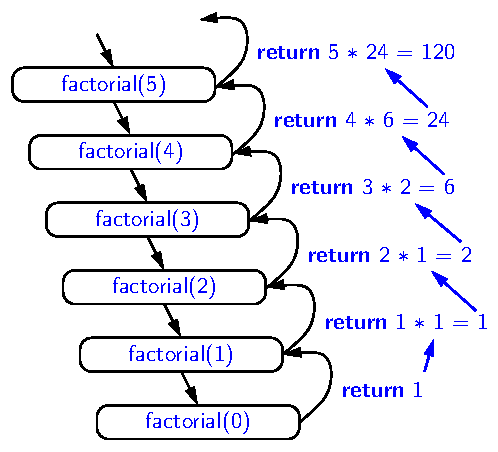
\includegraphics[width=7cm]{asp-02-pic01.pdf}
  \end{center}
}
\frame{
  \frametitle{Primer rekurzije: ,,engleski lenjir``}
  \begin{itemize}
    \item odštampati crtice i brojeve tako da se dobije izgled lenjira
  \end{itemize}
  \begin{center}
    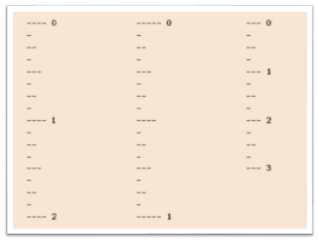
\includegraphics[width=8cm]{asp-02-pic02.png}
  \end{center}
}
\frame{
  \frametitle{Crtanje ,,engleskog lenjira``}
  \begin{itemize}
    \item \texttt{\myred{drawTicks}(length)}
    \item ulaz: dužina crtice
    \item izlaz: lenjir sa crticom date dužine u sredini i manji lenjiri sa leve
    i desne strane
  \end{itemize}
  \begin{center}
    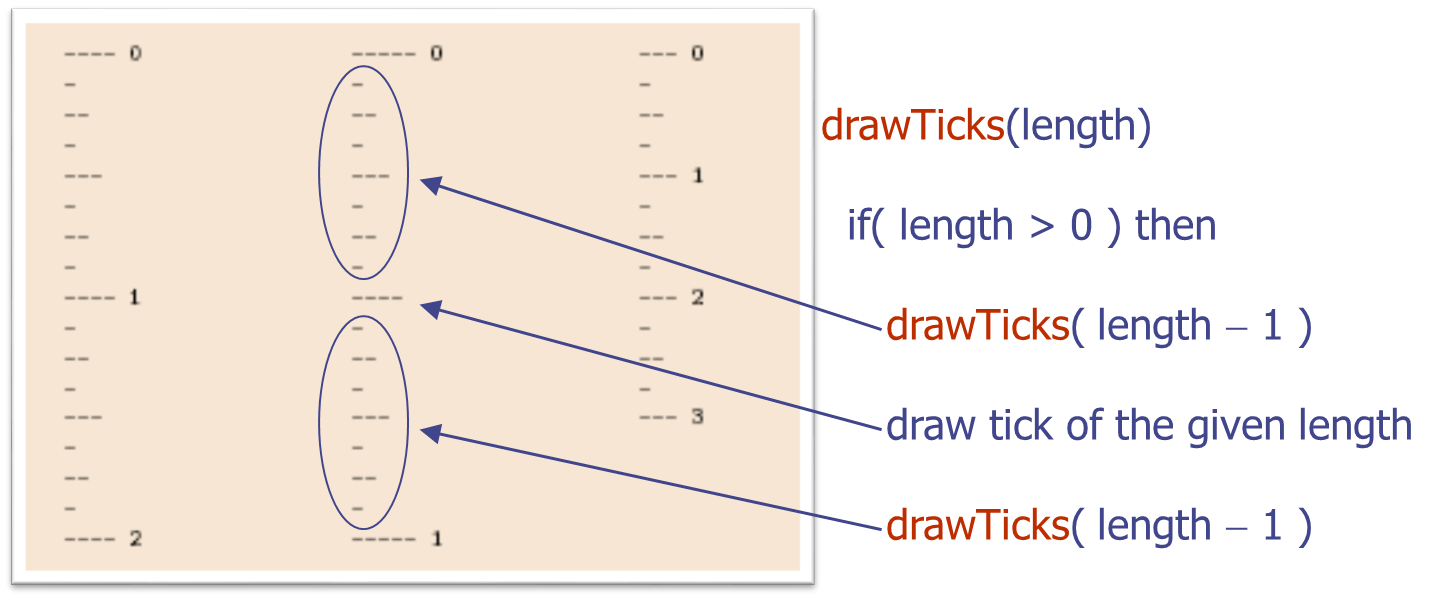
\includegraphics[width=11cm]{asp-02-pic03.png}
  \end{center}
}
\frame{
  \frametitle{Crtanje ,,engleskog lenjira``}
  \begin{itemize}
    \item interval sa centralnom crticom dužine $L \ge 1$ sastoji se od
    \begin{itemize}
      \item intervala sa centralnom crticom dužine $L-1$
      \item crtice dužine $L$
      \item intervala sa centralnom crticom dužine $L-1$
    \end{itemize}
  \end{itemize}
}
\frame{
  \frametitle{Crtanje ,,engleskog lenjira``}
  \begin{center}
    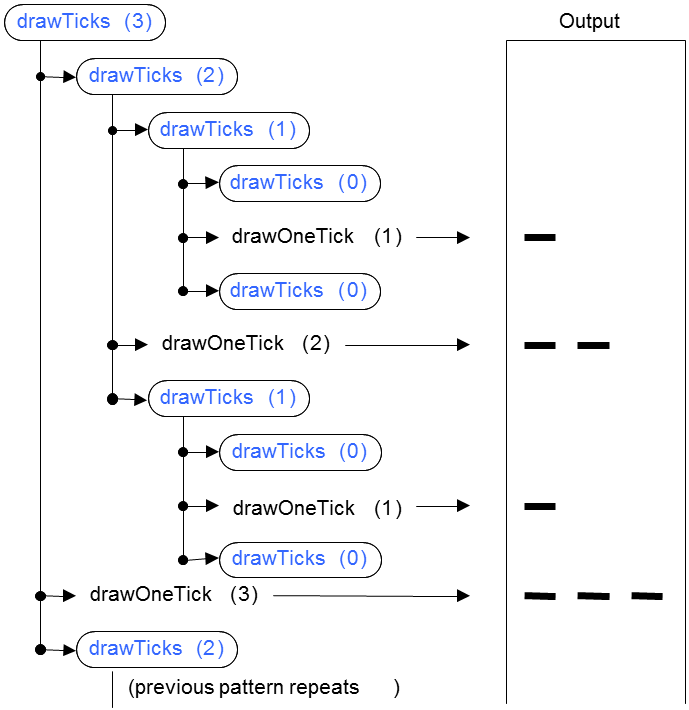
\includegraphics[width=7cm]{asp-02-pic04.png}
  \end{center}
}
\begin{frame}[fragile,shrink=10]
  \frametitle{Crtanje ,,engleskog lenjira``: Python implementacija}
\begin{minted}[linenos=false]{python}
def draw_line(tick_length, tick_label=''):
    """Draw one line with given tick length (followed by optional label)."""
    line = '-' * tick_length
    if tick_label:
        line += tick_label
    print(line)

def draw_interval(center_length):
    """Draw tick interval based upon a central tick length."""
    if center_length > 0:                 # recursively draw top ticks
        draw_interval(center_length - 1)  # draw center tick
        draw_line(center_length)          # recursively draw bottom ticks
        draw_interval(center_length - 1)

def draw_ruler(num_inches, major_length):
    """Draw English ruler with given number of inches, major tick length."""
    draw_line(major_length, '0')          # draw inch 0 line
    for j in range(1, 1+num_inches):
        draw_interval(major_length - 1)   # draw interior ticks for inch
        draw_line(major_length, str(j))   # draw inch j line and label
\end{minted}  
\end{frame}
\begin{frame}[fragile,shrink=15]
  \frametitle{Binarna pretraga}
\begin{minted}[linenos=false]{python}
def binary_search(data, target, low, high):
  """Return True if target is found in indicated portion of a Python 
  list. The search only considers the portion from data[low] to 
  data[high] inclusive.
  """
  if low > high:
    return False                    # interval is empty; no match
  else:
    mid = (low + high) // 2
    if target == data[mid]:         # found a match
      return True
    elif target < data[mid]:
      # recur on the portion left of the middle
      return binary_search(data, target, low, mid - 1)
    else:
      # recur on the portion right of the middle
      return binary_search(data, target, mid + 1, high)
\end{minted}  
\end{frame}
\end{document}
